\documentclass[11pt,a4paper]{article}
% Preámbulo común. Fuente: Calibri (se carga desde Windows). Si no la tienes, cambia la línea \setmainfont por "Carlito" (equivalente libre).
\usepackage[a4paper,margin=2cm,top=1.8cm,bottom=1.8cm]{geometry}
\usepackage{fontspec}
\setmainfont{calibri}[Path=/mnt/c/Windows/Fonts/,Extension=.ttf,UprightFont=*,BoldFont=*b,ItalicFont=*i,BoldItalicFont=*z]
\usepackage{microtype}
\usepackage{titlesec}
\usepackage{enumitem}
\usepackage{booktabs}
\usepackage{array}
\usepackage{tabularx}
\usepackage{graphicx}
\usepackage{fancyvrb}
\usepackage{fancyhdr}
\usepackage{xcolor}
\definecolor{negro}{rgb}{0,0,0}
\color{negro}
\pagestyle{fancy}\fancyhf{}\renewcommand{\headrulewidth}{0pt}
\fancyfoot[C]{\small\thepage}
\setlength{\parindent}{0pt}\setlength{\parskip}{4pt}
\titleformat{\section}{\large\bfseries}{\thesection.}{0.5em}{}
\titlespacing*{\section}{0pt}{9pt}{3pt}
\setlist{nosep,leftmargin=1.2em}
\renewcommand{\arraystretch}{1.15}

\geometry{margin=1.8cm,top=1.5cm,bottom=1.4cm}
\begin{document}
\pagestyle{empty}
{\Huge\bfseries Rescate en la Cueva}\\[2pt]
{\large Un juego de equipo para aprender a decidir bajo presión, con IA dentro de la partida}

\vspace{3pt}\hrule\vspace{5pt}

\begin{minipage}[t]{0.56\textwidth}
\textbf{¿Para quién es?}\\
Centros de FP y de formación de adultos que quieren trabajar la comunicación y el liderazgo con algo más vivo que una charla. También equipos de empresa y eventos de team building que buscan una actividad corta, de unos 15 minutos, que no necesite instalar nada.

\textbf{¿Qué problema resuelve?}\\
Las dinámicas de equipo suelen ser aburridas, hay que prepararlas y dependen de que alguien las dirija. Aquí el juego explica las reglas, cuenta la historia y dirige la partida solo, y al final cada jugador puede ver qué decisiones tomó y en qué influyeron.

\textbf{¿Qué ofrece?}
\begin{itemize}
\item Tres roles con información privada y objetivos distintos, así que hay que hablar, confiar y a veces desconfiar.
\item Cinco tramos con decisiones que cambian la ruta y el final.
\item Un diario al acabar cada tramo que enseña qué decidió cada uno y qué consecuencias tuvo.
\item Se juega en el navegador, en ordenador o móvil, solo o con amigos por enlace o QR.
\end{itemize}
\end{minipage}\hfill
\begin{minipage}[t]{0.40\textwidth}
\vspace{0pt}
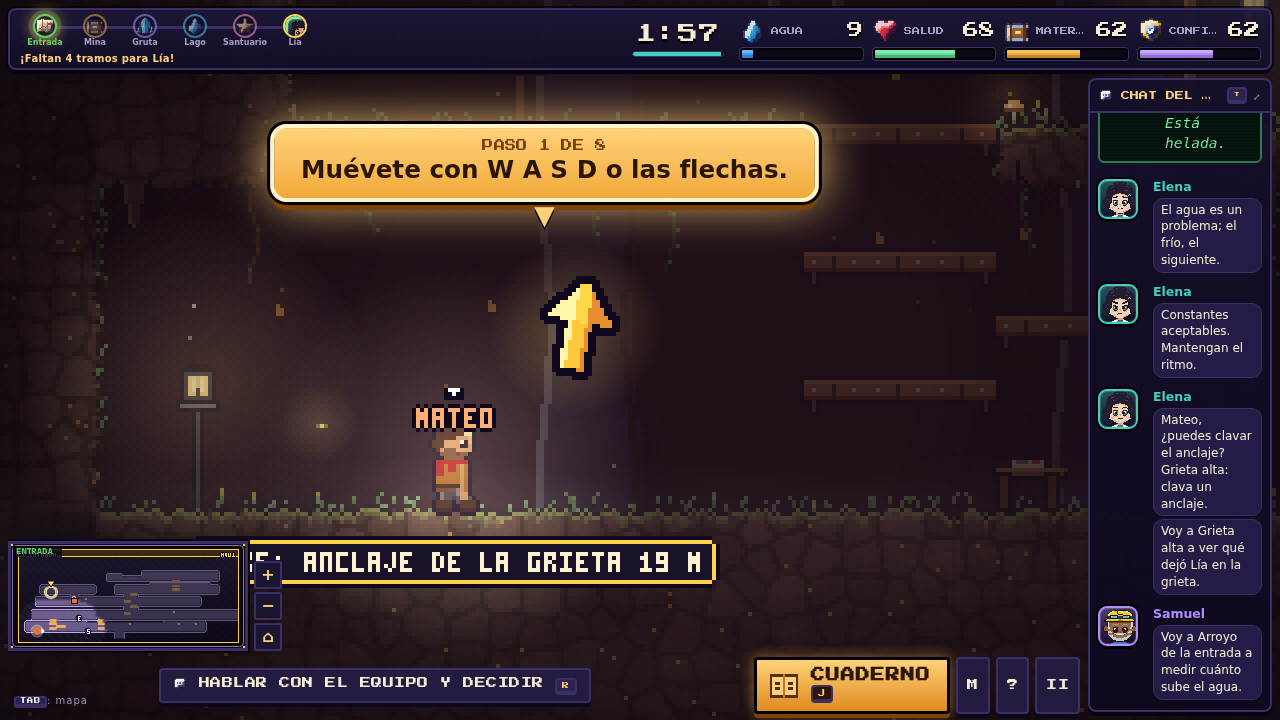
\includegraphics[width=\textwidth]{captura.png}\\[-1pt]
{\footnotesize Captura de la partida}
\end{minipage}

\vspace{4pt}
\textbf{¿Qué lo diferencia de un juego normal?}
\begin{itemize}
\item \textbf{La IA forma parte del juego.} Hay un director que cuenta cada tramo, compañeros que conversan y deciden por su cuenta y un árbitro que explica el resultado. Reciben el estado de la partida y su información privada, y el código comprueba todo lo que responden para que no rompan las reglas.
\item \textbf{Información asimétrica:} cada jugador sabe cosas distintas, y se puede mentir.
\item \textbf{Funciona aunque falle la IA o internet:} hay un modo demo sin clave, así que una clase nunca se queda sin actividad.
\item \textbf{Sin servidor propio:} las partidas online son entre navegadores, por eso es barato de mantener.
\end{itemize}

\textbf{Modelo de acceso (propuesta, todavía no implementada)}
\begin{itemize}
\item \textbf{Gratis:} modo demo, sin IA.
\item \textbf{Licencia por centro o por curso:} incluye la IA y un panel para que el profesor vea los resultados de la clase.
\item \textbf{Pago por sesión} para empresas y eventos, con la partida preparada para su equipo.
\end{itemize}

\textbf{Cómo probarlo}\\
Juego: https://francodavidgc366-wq.github.io/rescate-cueva/\\
Código: https://github.com/francodavidgc366-wq/rescate-cueva

\vspace{2pt}
{\small Franco David García Coral · MP3 · Programació d'Intel·ligència Artificial · 22 de octubre de 2026}
\end{document}
